\section{Business to Business (B2B)}
This application was built from the ground up for a large clothes manufacturer, who sells boxes of clothes to thousands of stores in 30+ markets. It replaces a manual process, where travelling salesmen visited the stores and presented physical clothing from their sample collections.

The \gls{b2b} order application enables the clients, e.g. shop employees, to see a catalogue of upcoming clothes on a tablet device, and place orders on boxes for future delivery, shown in Table \ref{tab:b2b_constants_variables}. This functionality is made available for the same shops to shop staff as well as for shop managers, managers of chains of shops or managers of entire markets.
\begin{table*}[!ht]
	\begin{tabular}{|p{2.4cm}|p{13.2cm}|r| }
		\hline
			\multicolumn{1}{|c|}{Name} & \multicolumn{1}{c|}{Description} & \multicolumn{1}{c|}{Type} \\
		\hline
		\hline
			$Business_{d}$ & It is the set of businesses as seen by the \gls{dc} $d$ and $b$ represents one of those businesses, $b \in Businesses$. &  \\
		\hline
			$Clothes_{db}$ & It is the set of clothes for business $b$ as seen by the \gls{dc} $d$ and $l$ represents one of those clothes, $l \in Clothes_{b}$. & \\
		\hline
			$Cost_{dbl}$ & It is the cost of a box of clothes $l$ from business $b$ as seen by the \gls{dc} $d$. & $\mathbb{R}_{+}$ \\
		\hline
			$Capacity_{dbl}$ & It is the maximum quantity of available boxes of clothes $l$ as seen by the \gls{dc} $d$. &  $\mathbb{Z}_{+}$ \\
		\hline
			$Clients_{db}$ & It is the set of clients for business $b$ as seen by the \gls{dc} $d$ and $c$ represents one of those clients, $c \in Clients_{b}$. & \\
		\hline
			$Credit_{dbc}$ & It is the credit of client $c$ from business $b$ as seen by the \gls{dc} $d$. & $\mathbb{R}$ \\
		\hline
			$Boxes_{dblc}$ & It is the number of boxes of clothes $l$ from business $b$ ordered by client $c$ as seen by the \gls{dc} $d$. & $\mathbb{Z}_{+}$ \\
		\hline
	\end{tabular}
	
	\caption{\gls{b2b} Constants and Variables.}
	\label{tab:b2b_constants_variables}
\end{table*}

{\bf Constraints} for this problem:\\
It is not allowed to order more boxes for a particular clothe $c$ from a business $b$ between all the clients of that business than those available $Capacity_{dbl}$, but less may be ordered as expressed in Inequality \ref{inq:b2b_clothes_total}.
\begin{equation} \label{inq:b2b_clothes_total}
	Caplcity_{dbl} \ge \sum_{c \in Clients_{db}} Boxes_{dblc}
\end{equation}

It is not allowed to expend by any of the clients in orders more that their credit from business $b$ as expressed by Inequality \ref{inq:b2b_max_expent}.
\begin{equation} \label{inq:b2b_max_expent}
	Credit_{dbc} \ge \sum_{l \in Clothes_{db}} (Boxes_{dblc} * Cost_{dbl})
\end{equation}

Orders are modelled as a \gls{gset} \cite{shapiro11comprehensive}, which is updated by adding event objects.

The tablets can operate off-line and only need to be online for getting i.e. new catalogue replicated down and for posting orders towards the server. It is expected that stores cannot be spread over many \glspl{dc}. More \glspl{dc} can be used and in this case each \gls{dc} must be aware of in which \gls{dc} each shop's data is located.

The tablets can remain off-line for any length of time. This effectively means that there will be issues with double orders, out of stock, not current catalogue, and other conflicts. The automated system is not intended for handling these conflicts while it will attempt to detect conflicts and potential conflicts. These will then be brought to the attention of manufacturer's customer support.

Cancellation and adjustment of orders are not offered via the tablet solution. These will have to be dealt with by the manufacturers customer support. An overall view of the system can be seen in Figure \ref{fig:b2b_architecture}.
\begin{figure*}[ht!]
	\centering
	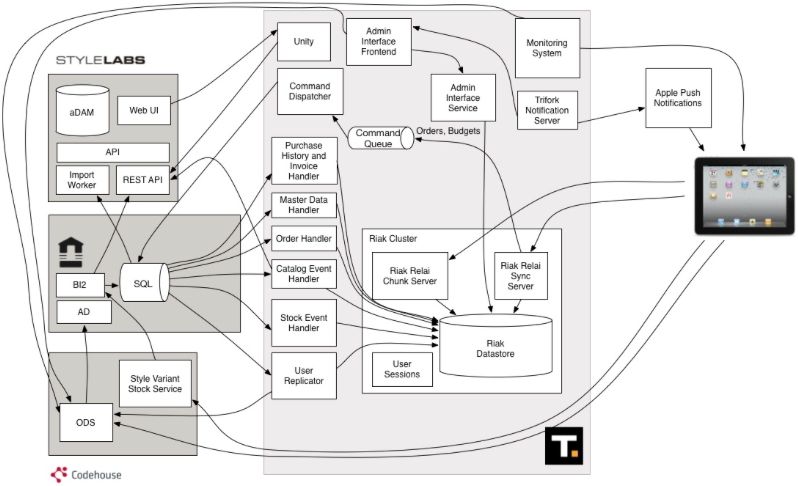
\includegraphics[width=1\textwidth]{figures/b2b.png}
	
	\caption{B2B eCommerce Architecture (P2tF).}
	\label{fig:b2b_architecture}
\end{figure*}
